% Data and state assignments: 277Cn_decay_scheme_codex.md.
% Layout: supplied Haba reference image, extended upward to Cn.
% Compile with: pdflatex 277Cn_full_decay_scheme.tex
\documentclass[tikz,border=6pt]{standalone}
\usepackage{amsmath}
\usepackage{newtxtext,newtxmath}
\usetikzlibrary{arrows.meta,calc}

% Change to \draftnotesfalse to hide the provisional branch-ratio note.
\newif\ifdraftnotes
\draftnotestrue

\definecolor{nuclideyellow}{HTML}{F7E900}
\definecolor{fissiongreen}{HTML}{70B941}

\tikzset{
  box edge/.style={draw, line width=0.8pt},
  nuc/.style={
    box edge, fill=nuclideyellow, minimum size=2.5cm,
    inner sep=0pt, outer sep=0pt
  },
  main decay/.style={line width=0.8pt, -{Straight Barb[length=2.5mm,width=2mm]}},
  minor decay/.style={main decay, densely dotted},
  isotope label/.style={font=\fontsize{25}{25}\selectfont, inner sep=0pt},
  state label/.style={font=\fontsize{14}{15}\selectfont, inner sep=0pt},
  decay label/.style={font=\fontsize{11}{13}\selectfont, align=center, inner sep=1pt}
}

\newcommand{\isotope}[2]{{}^{#1}\mathrm{#2}}

% The same square and type sizes are used throughout all six levels.
\newcommand{\singlestate}[5]{%
  \node[nuc] (#1) at (#2,#3) {};
  \node[isotope label] at ($(#1.north)+(0,-0.80)$) {$#4$};
  \node[state label] at ($(#1.south)+(0,0.53)$) {$#5$};
}

% Add the common labels and connection points to an existing square.
\newcommand{\doublestate}[7][]{%
  \node[isotope label] at ($(#2.north)+(0,-0.73)$) {$#3$};
  \draw[box edge] (#2.south) -- ++(0,1.20);
  \node[state label] at ($(#2.south)+(-0.625,0.93)$) {$\boldsymbol{#4}$};
  \node[state label] at ($(#2.south)+( 0.625,0.93)$) {$\boldsymbol{#5}$};
  \node[state label,#1] at ($(#2.south)+(-0.625,0.36)$) {$#6$};
  \node[state label,#1] at ($(#2.south)+( 0.625,0.36)$) {$#7$};
  \coordinate (#2-left-in)   at ($(#2.north)+(-0.625,0)$);
  \coordinate (#2-right-in)  at ($(#2.north)+( 0.625,0)$);
  \coordinate (#2-left-out)  at ($(#2.south)+(-0.625,0)$);
  \coordinate (#2-right-out) at ($(#2.south)+( 0.625,0)$);
}

\begin{document}
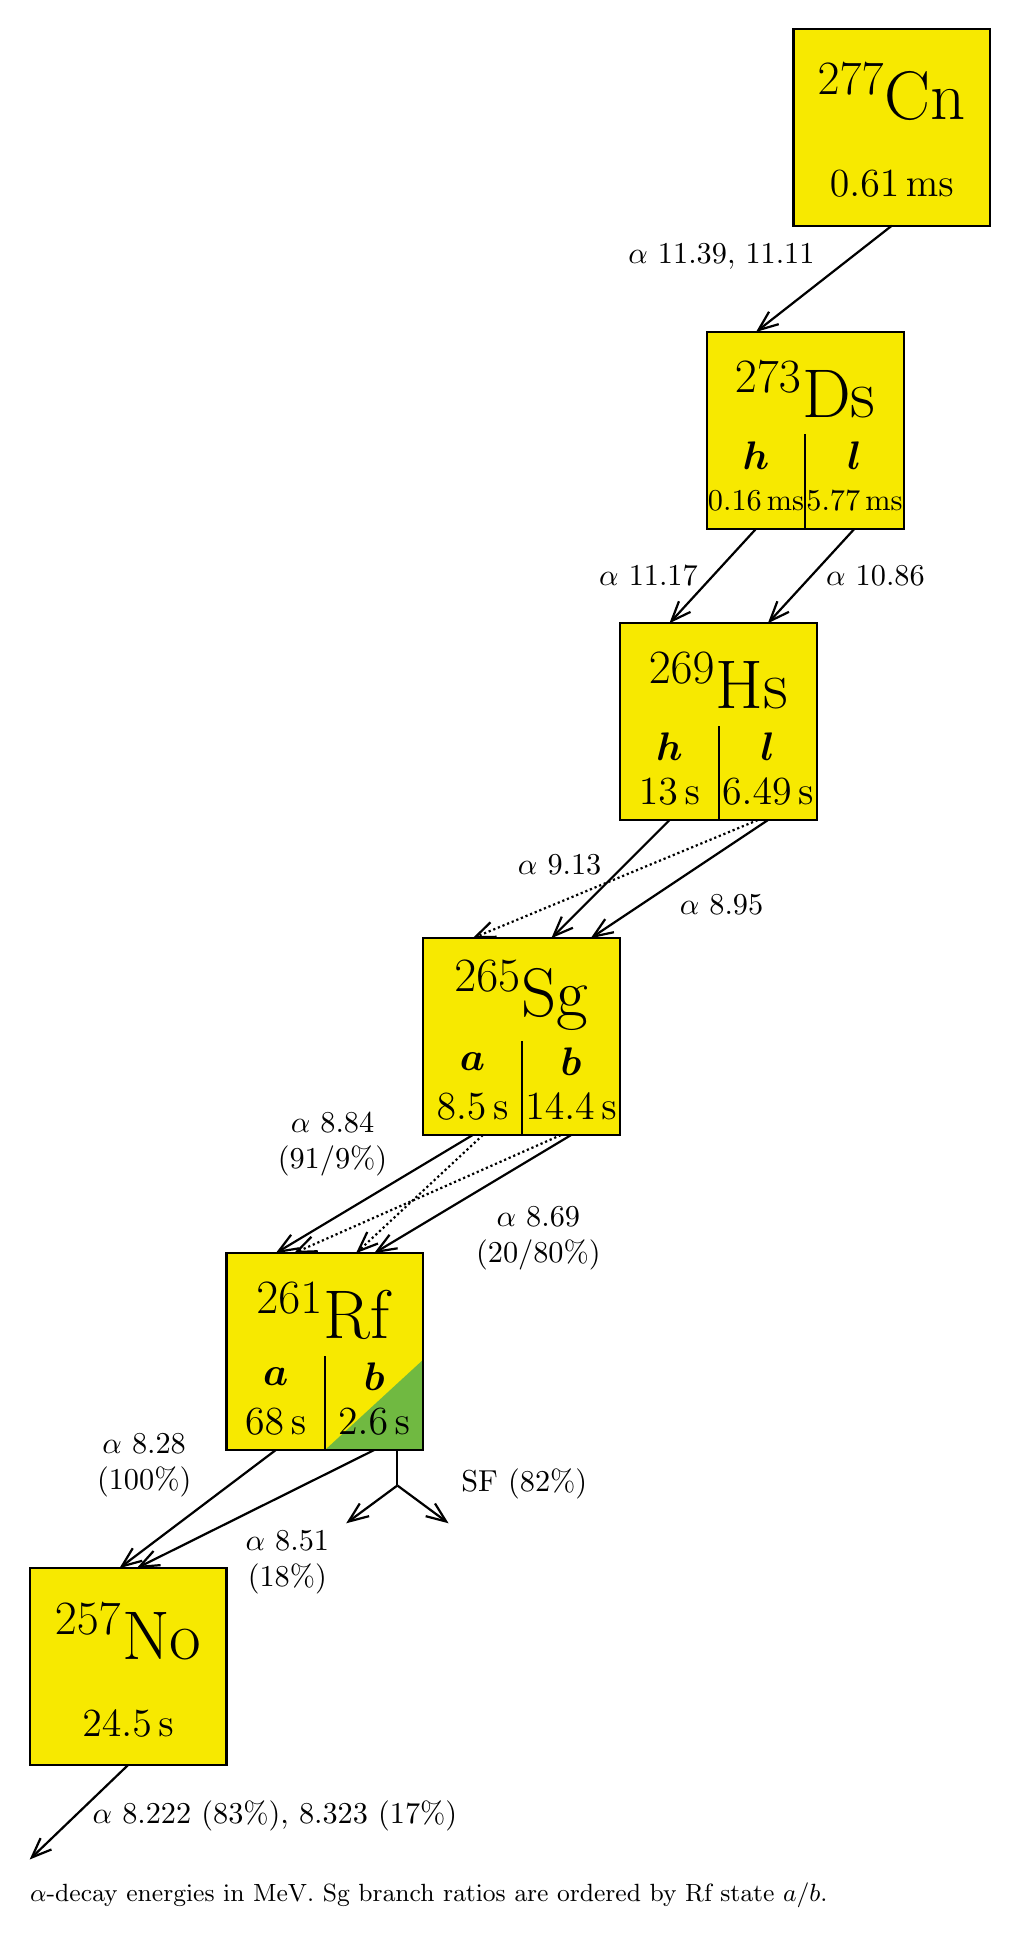
\begin{tikzpicture}
  \singlestate{cn}{5.25}{0}{\isotope{277}{Cn}}{0.61\,\mathrm{ms}}
  \node[nuc] (ds) at (4.15,-3.85) {};
  \doublestate[font=\fontsize{10.5}{12}\selectfont]{ds}{\isotope{273}{Ds}}{h}{l}
    {0.16\,\mathrm{ms}}{5.77\,\mathrm{ms}}
  \node[nuc] (hs) at (3.05,-7.55) {};
  \doublestate{hs}{\isotope{269}{Hs}}{h}{l}{13\,\mathrm{s}}{6.49\,\mathrm{s}}

  % The Sg, Rf and No centres step left by one box width per level.
  \node[nuc] (sg) at (0.55,-11.55) {};
  \doublestate{sg}{\isotope{265}{Sg}}{a}{b}{8.5\,\mathrm{s}}{14.4\,\mathrm{s}}
  \node[nuc] (rf) at (-1.95,-15.55) {};
  \fill[fissiongreen] (rf.south) -- (rf.south east) -- ++(0,1.15) -- cycle;
  \draw[box edge] (rf.south west) rectangle (rf.north east);
  \doublestate{rf}{\isotope{261}{Rf}}{a}{b}{68\,\mathrm{s}}{2.6\,\mathrm{s}}
  \singlestate{no}{-4.45}{-19.55}{\isotope{257}{No}}{24.5\,\mathrm{s}}

  % CHECK A: both Cn energies provisionally feed Ds^h as supplied.
  % The upstream population of Ds^l is unspecified. Its path starts at Ds^l.
  \draw[main decay] (cn.south) --
    node[decay label,above left=2pt] {$\alpha\ 11.39,\,11.11$} (ds-left-in);

  \draw[main decay] (ds-left-out) --
    node[decay label,left=4pt] {$\alpha\ 11.17$} (hs-left-in);
  \draw[main decay] (ds-right-out) --
    node[decay label,right=4pt] {$\alpha\ 10.86$} (hs-right-in);

  % Additional minor path requested from Hs^l to Sg^a.
  % Its branching ratio has not been assigned in the input.
  \draw[minor decay] ($(hs-right-out)+(-0.13,0)$) -- (sg-left-in);
  \draw[main decay] (hs-left-out) --
    node[decay label,above left=1pt,pos=0.52] {$\alpha\ 9.13$}
    ($(sg-right-in)+(-0.25,0)$);
  % CHECK B: both 86%/14% entries originally name Sg^b. The allocation
  % of those percentages between the solid and dotted paths is pending.
  \draw[main decay] (hs-right-out) --
    node[decay label,below right=2pt,pos=0.55] {
      $\alpha\ 8.95$%
      \ifdraftnotes\\(14/86\%)\fi
    } ($(sg-right-in)+(0.25,0)$);

  % Ratios are ordered by the Rf destination, a/b. Separate the minor
  % arrow tips slightly so the four connections remain visible in print.
  \draw[minor decay] ($(sg-left-out)+(0.13,0)$) -- ($(rf-right-in)+(-0.23,0)$);
  \draw[minor decay] ($(sg-right-out)+(-0.13,0)$) -- ($(rf-left-in)+(0.23,0)$);
  \draw[main decay] (sg-left-out) --
    node[decay label,above left=1pt,pos=0.40] {$\alpha\ 8.84$\\(91/9\%)} (rf-left-in);
  \draw[main decay] (sg-right-out) --
    node[decay label,below right=2pt,pos=0.53] {$\alpha\ 8.69$\\(20/80\%)} (rf-right-in);

  \draw[main decay] (rf-left-out) --
    node[decay label,above left=2pt,pos=0.48] {$\alpha\ 8.28$\\(100\%)}
    ($(no.north)+(-0.11,0)$);
  \draw[main decay] (rf-right-out) -- ($(no.north)+(0.11,0)$);
  \node[decay label,anchor=west] at ($(no.north east)+(0.20,0.07)$) {$\alpha\ 8.51$\\(18\%)};

  % A forked arrow indicates the single spontaneous-fission branch.
  \draw[line width=0.8pt] ($(rf.south)+(0.92,0)$) -- ++(0,-0.45) coordinate (sf);
  \draw[main decay] (sf) -- ++(-0.65,-0.48);
  \draw[main decay] (sf) -- ++( 0.65,-0.48);
  \node[decay label,right=2pt] at ($(sf)+(0.70,0.02)$) {SF (82\%)};

  \draw[main decay] (no.south) -- ++(-1.25,-1.20)
    node[decay label,right=5pt,pos=0.54] {$\alpha\ 8.222$ (83\%), $8.323$ (17\%)};

  \node[font=\small,align=left,anchor=west,inner sep=0pt] at (-5.7,-22.45) {
    $\alpha$-decay energies in MeV. Sg branch ratios are ordered by Rf state $a/b$.
  };
\end{tikzpicture}
\end{document}
